\documentclass{article}
\usepackage{blindtext}
\usepackage[english]{babel}
\usepackage[T1]{fontenc}
\usepackage[utf8]{inputenc}

\usepackage{import}
\usepackage{pgfplots}
\usepackage{pgf-pie/pgf-pie}
\usepackage{tikz}
\usepackage{chemfig}
\begin{document}


\begin{titlepage}
  \centering
 

  \vspace{0.5cm}
  {\scshape\Large department \par}
  \vspace{1.5cm}
  {\huge\bfseries Subject \par}
  \vspace{2cm}
  {\Large {\fontfamily{ptm}\selectfont writer } \par}
  \vfill

lecture name \textsc{last name}

  \vfill

  % Bottom of the page
  {\large 26 Kasım 2020\par}
\end{titlepage}
\newpage


\tableofcontents
\listoffigures
\listoftables
\newpage
\section{Giriş}

Lorem Ipsum is simply dummy text of the printing and typesetting industry. Lorem Ipsum has been the industry's standard dummy text ever since the 1500s, when an unknown printer took a galley of type and scrambled it to make a type specimen book. It has survived not only five centuries, but also the leap into electronic typesetting, remaining essentially unchanged. It was popularised in the 1960s with the release of Letraset sheets containing Lorem Ipsum passages, and more recently with desktop publishing software like Aldus PageMaker including versions of Lorem Ipsum 
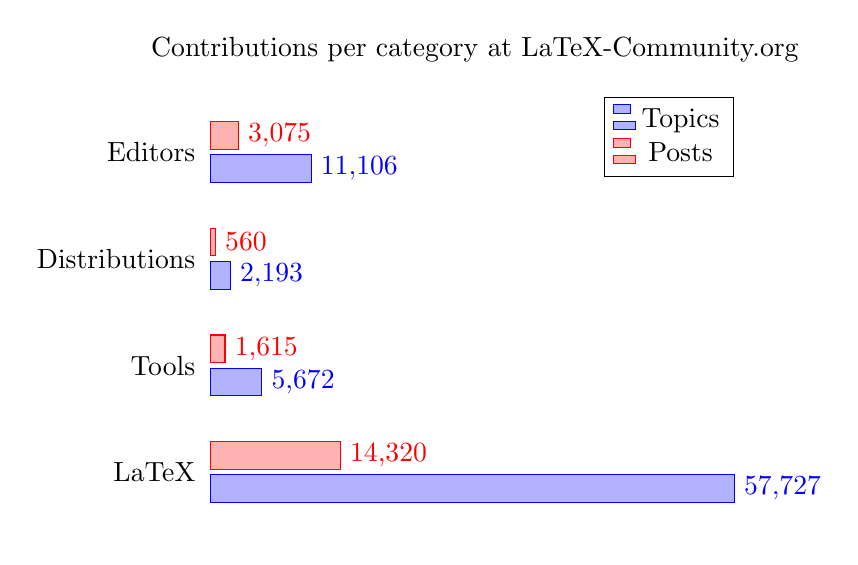
\begin{tikzpicture}
  \begin{axis}
[
    title    = Contributions per category
               at LaTeX-Community.org,
    xbar,
    y axis line style = { opacity = 0 },
    axis x line       = none,
    tickwidth         = 0pt,
    enlarge y limits  = 0.2,
    enlarge x limits  = 0.02,
    nodes near coords,
    symbolic y coords = {LaTeX, Tools,
                         Distributions, Editors},
  ]
  \addplot coordinates { (57727,LaTeX) (5672,Tools)
           (2193,Distributions) (11106,Editors) };
  \addplot coordinates { (14320,LaTeX) (1615,Tools)
           (560,Distributions)  (3075,Editors)  };
             \legend{Topics, Posts}

               \end{axis}
\end{tikzpicture}

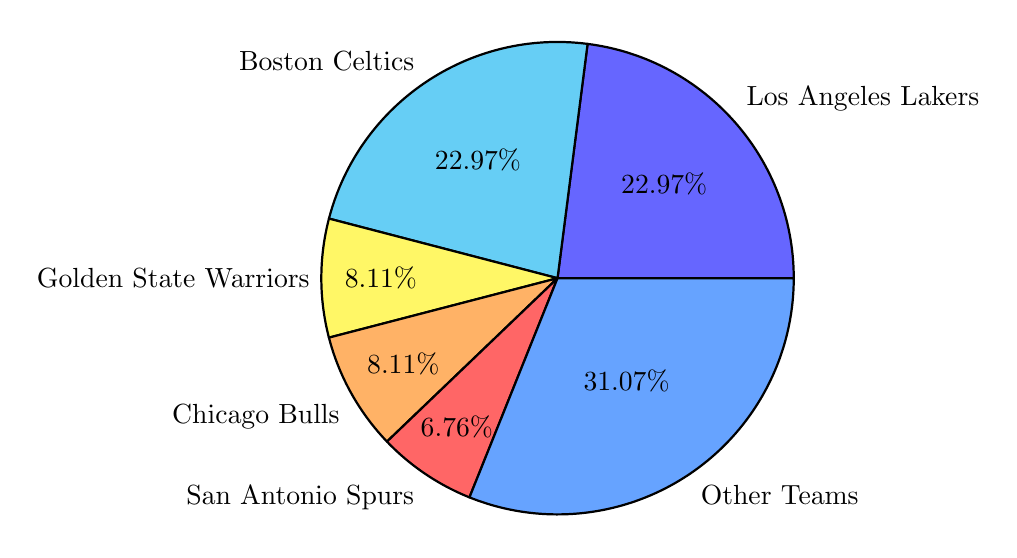
\begin{tikzpicture}

\pie{22.97/Los Angeles Lakers,
    22.97/Boston Celtics,
    8.11/Golden State Warriors,
    8.11/Chicago Bulls,
    6.76/San Antonio Spurs,
    31.07/Other Teams}

\end{tikzpicture}

Regular polygons

\chemfig{A*5(-B=C-D-E=)}

Incomplete rings are also possible

\chemfig{A*5(-B=C-D)}

\end{document}